% !TEX TS-program = pdflatex
% !TEX encoding = UTF-8 Unicode

% This is a simple template for a LaTeX document using the "article" class.
% See "book", "report", "letter" for other types of document.

\documentclass[11pt]{article} % use larger type; default would be 10pt

\usepackage[utf8]{inputenc} % set input encoding (not needed with XeLaTeX)

%%% Examples of Article customizations
% These packages are optional, depending whether you want the features they provide.
% See the LaTeX Companion or other references for full information.

%%% PAGE DIMENSIONS
\usepackage{geometry} % to change the page dimensions
\geometry{a4paper} % or letterpaper (US) or a5paper or....
% \geometry{margin=2in} % for example, change the margins to 2 inches all round
% \geometry{landscape} % set up the page for landscape
%   read geometry.pdf for detailed page layout information

\usepackage{graphicx} % support the \includegraphics command and options

% \usepackage[parfill]{parskip} % Activate to begin paragraphs with an empty line rather than an indent

%%% PACKAGES
\usepackage{booktabs} % for much better looking tables
\usepackage{array} % for better arrays (eg matrices) in maths
%\usepackage{paralist} % very flexible & customisable lists (eg. enumerate/itemize, etc.)
\usepackage{verbatim} % adds environment for commenting out blocks of text & for better verbatim
\usepackage{subfig} % make it possible to include more than one captioned figure/table in a single float
% These packages are all incorporated in the memoir class to one degree or another...

%%% HEADERS & FOOTERS
\usepackage{fancyhdr} % This should be set AFTER setting up the page geometry
\pagestyle{fancy} % options: empty , plain , fancy
\renewcommand{\headrulewidth}{0pt} % customise the layout...
\lhead{}\chead{}\rhead{}
\lfoot{}\cfoot{\thepage}\rfoot{}

%%% SECTION TITLE APPEARANCE
\usepackage{sectsty}
\allsectionsfont{\sffamily\mdseries\upshape} % (See the fntguide.pdf for font help)
% (This matches ConTeXt defaults)

%%% ToC (table of contents) APPEARANCE
\usepackage[nottoc,notlof,notlot]{tocbibind} % Put the bibliography in the ToC
\usepackage[titles,subfigure]{tocloft} % Alter the style of the Table of Contents
\renewcommand{\cftsecfont}{\rmfamily\mdseries\upshape}
\renewcommand{\cftsecpagefont}{\rmfamily\mdseries\upshape} % No bold!

%%% END Article customizations
\usepackage{url}
\usepackage[spanish]{babel}
\usepackage{listings} 
%%% The "real" document content comes below...

\title{XML PARSER}
%\date{} % Activate to display a given date or no date (if empty),
         % otherwise the current date is printed 
         
\author{Edinson Sanchez\\Kevin Filella\\Adrian Aguilar}

\begin{document}
\maketitle

%----------------------------------------------------------------------------------------
%	TABLE OF CONTENTS
%----------------------------------------------------------------------------------------

%\setcounter{tocdepth}{1} % Uncomment this line if you don't want subsections listed in the ToC

\newpage
\tableofcontents
\newpage

\section{Introducción}
Un parser, aplicado a lenguajes de programación computacionales, tiene como objetivo el de manipular ciertas cadenas de caracteres con el fin de asignar o guardar la información presentada en una estructura de datos.
Una vez conocido esto, el objetivo de este proyecto es claro y conciso; el de crear un parser XML en Pythonl que pueda manipular, leer y guardar los datos presentados en un archivo XML específico, con una estructura fija y con un propósito previsto; el de realizar consultas a la estructura.


\subsection{Objetivo}
Nuestro objetivo en este proyecto es el de crear un parser XML en Pythonl que pueda manipular, leer y guardar los datos presentados en un archivo XML específico, con una estructura fija y con un propósito previsto; el de realizar consultas a la estructura.

\section{Desarrollo}
\subsection{Desarrollo inicial}
Inicialmente, debido a la naturaleza del proyecto y a las características del curso presente, tuvimos que aprender a instalar y manejar las herramientas de desarrollo adecuadas. Siendo este lenguaje funcional y de uso masivo fue muy fácil instalar las herramientas adecuadas y empezar a programar en Python.

\section{Problemas}


Problemas en el aprendizaje e implementación del lenguaje Python a la creación de un parser XML.



\subsection{Primer Problema - Sintaxis}

Al momento de iniciar el curso de lenguajes de programación, nosotros como estudiantes, debido al programa de estudios, hemos sido iniciados en algunos lenguajes de programación. Lenguajes como Pascal, BASIC, C, C++, Java, Android etc. Estos lenguajes son todos de alguna manera u otra muy similares entre sí. Python es un lenguaje funcional con características muy similares a los lenguajes anteriormente mencionados. Lo que hizo bastante fácil el trabajo de aprender el correcto uso de la sintaxis en Python. El  único aspecto un poco confuso es la estricta rigurosidad del lenguaje en cuanto a la indentación de las líneas.


\subsection{Segundo Problema - Estructura}

Como este proyecto ya había sido realizado anteriormente en lenguaje Haskell, este proyecto en principio parecía simplemente un trabajo de traducción. Por lo cual decidimos implementar una estructura similar a la del proyecto anterior. Esta labor en principio sencilla en etapas posteriores del desarrollo demostraría ser una mala elección de diseño, ya que en Haskell todo lo resolvíamos recursivamente mientras que Python no maneja tan bien la recursividad. 

\subsection{Tercer Problema - Recursividad}

El hecho de que Python maneje la recursividad de una manera muy distinta a la de Haskell fue el problema más grande en el desarrollo de este proyecto. Python guarda la salida de cada función recursiva en una pila de tamaño limitado. Puede guardar hasta 14000 líneas de recursión, Esto es un problema irresoluble cuando se quiere parsear documentos de gran tamaño.



\subsection{Cuarto Problema - Busquedas}

El parseo del documento se lo tuvo que realizar iterativamente, línea por línea, lo que demora algunos segundos lo cual es demasiado tiempo. Pero para el alcance y las limitaciones de este proyecto podría ser incluso aceptable. El problema mayos se daría cuando realizamos las búsquedas en la lista de devices que grabamos. Debido a que no pudimos aplicar recursividad en el parseo inicial los devices quedaron guardados en una larga lista sin orden aparente.

La búsqueda en una estructura tan grande consume demasiado tiempo, en el orden de las decimas de minutos, por lo cual intentamos forzar la recursividad utilizando una librería que aumenta l límite de líneas de recursividad que permite nativamente Python. Pero debido a la poca experiencia con este lenguaje y más aun con esta librería no estándar no pudimos hacer un uso correcto de la misma ni implementar búsqueda con recursión. 

\section{Alcance del Proyecto}


Al final nuestro proyecto tiene un alcance incompleto, más que nada debido a la falta de tiempo, experiencia y al hecho de que perdimos muchos días tratando de traducir el proyecto que habíamos realizado anteriormente en Haskell a Python. Nuestro proyecto puede realizar búsquedas lineales como devices que tengan un determinado fallback o determinadas características(capabilities). No puede realizar búsquedas recursivas como producir toda la línea de devices hasta llegar a generic. 


\section{Manual de uso}

Nuestro proyecto se puede ejecutar directamente desde el command prompt. Tal como se muestra en la imagen lo primero en mostrarse es un pequeño menú mostrando los créditos del proyecto y el menú principal , en el cual uno puede escoger entre las opciones de búsqueda, sea por fallback, por capability, o por release date. En este ejemplo el usuario procede a buscar devices por su reléase date, opción 3. Solo se debe escribir 3 y aplastar enter.

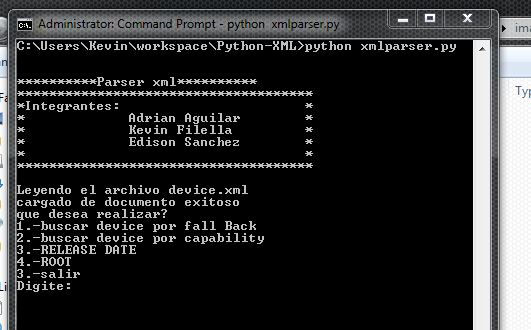
\includegraphics[width=13cm,height=11cm]{imagenes/mprincipal.jpg}


El programa te pregunta la reléase date que deseas ingresar para buscar en el archivo .En este caso deseamos encontrar todos los devices con release date 2011. Digitamos 2011 y presionamos enter, tras lo cual se proceden a imprimir en pantalla todos los devices con esta característica.


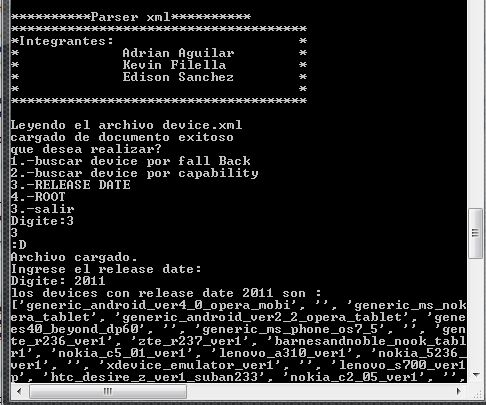
\includegraphics[width=13cm,height=10cm]{imagenes/usandorelease.jpg}

Luego que se imprimen todos los devices con release date 2011, el programa cuenta cuantos devices son en total y muestra el resultado. Tal como se muestra a continuación. 

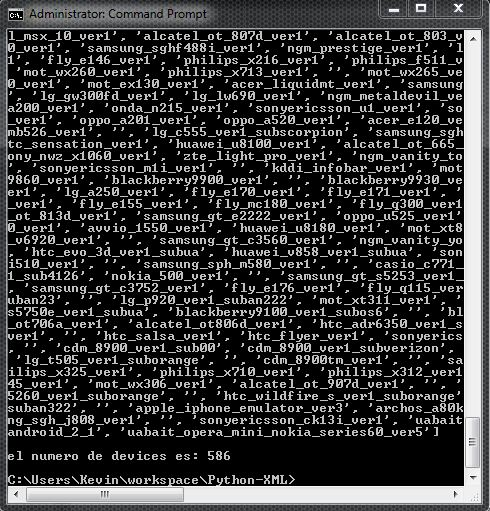
\includegraphics[width=13cm,height=11cm]{imagenes/numeroresultado.jpg}


\section{Conclusiones}

Como conclusión podemos decir que Haskell es un lenguaje mucho más efectivo para hacer parseo de grandes estructuras que Python. La forma iterativa de realizar las operaciones y el límite del tamaño que tiene la pila de recursión hacen muy difícil la tarea de realizar búsquedas grandes.
Python tiene una sintaxis muy fácil de aprender y utilizar, además que es un lenguaje muy flexible en el que puedes importar librerías de otros lenguajes, lo que lo hace ideal para programar cuando se requiere capacidad multiplataforma.













  


\end{document}